\vspace{1.5cm}


En la figura~\figref{fig:fig_p6_output_voltage} se muestra el gráfico de la tensión de salida en modo de regulación de tensión en función de la resistencia del resistor $R_{9}$, el gráfico se obtuvo realizando una simulación paramétrica con $R_{L} = 1 \si[per-mode=symbol]{\mega\ohm}$, con el comando \textbf{SPICE} \textit{.step}, y luego se exportó el resultado y se graficó en \textbf{MATLAB}. En el gráfico se puede apreciar que, como se espera según lo calculado, el crecimiento es lineal con $R_{9}$, entre valores muy cercanos a los nominales de $1 \si[per-mode=symbol]{\volt}$ y $10 \si[per-mode=symbol]{\volt}$.




\vfill

\clearpage

\begin{figure}[H] %htb
\begin{center}
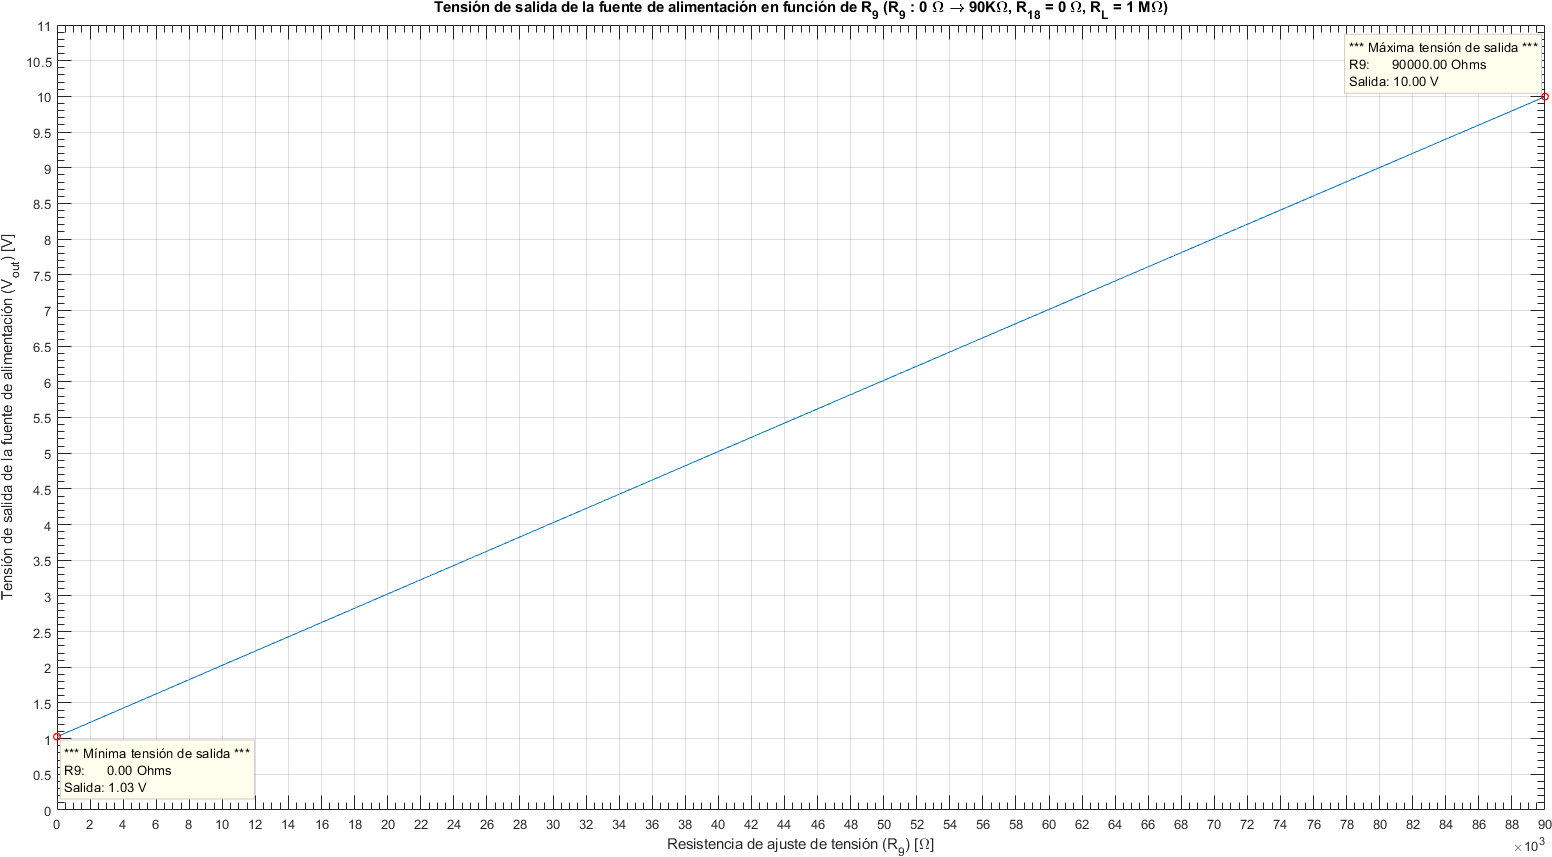
\includegraphics[width=1.2 \textwidth, angle=90]{./img/preguntas/p6.png}
\caption{\label{fig:fig_p6_output_voltage}\footnotesize{Tensión de salida, $V_{o}$, en función de $R_{9}$, con esta variando entre $0 \si[per-mode=symbol]{\ohm}$ y $90 \si[per-mode=symbol]{\kilo\ohm}$.}}
\end{center}
\end{figure}



\clearpage